\documentclass[12pt,letterpaper]{article}
\usepackage{amsmath}
\usepackage{amssymb}
\usepackage[round]{natbib}
\usepackage[left =1.0in,right=1.0in,top=1.0in,bottom=1.0in]{geometry}
\usepackage{graphicx}
\usepackage{nomencl}                    % produces a nomenclature
\usepackage{float}                      % figure floats
\usepackage{natbib}                     % this package allows you to link your references
\usepackage{graphicx}					% graphics package
\graphicspath{ {figures/}{figures/eps/}{figures/pdf/} }% specify the path where figures are located
\usepackage{fancyhdr}                   % fancy headers and footers
\usepackage{url}                        % nicely format url breaks
\usepackage[inactive]{srcltx}		 	% necessary to use forward and inverse searching in DVI
\usepackage{relsize}                    % font sizing hierarchy
\usepackage{booktabs}                   % professional looking tables
\usepackage[config, labelfont={bf}]{caption,subfig} % nice sub figures
\usepackage{mathrsfs}
\usepackage{amsmath}
\usepackage{amssymb}
\usepackage{threeparttable}	%footnote at bottom
\usepackage{array}
\newcolumntype{L}[1]{>{\raggedright\let\newline\\\arraybackslash\hspace{0pt}}m{#1}}
\newcolumntype{C}[1]{>{\centering\let\newline\\\arraybackslash\hspace{0pt}}m{#1}}
\newcolumntype{R}[1]{>{\raggedleft\let\newline\\\arraybackslash\hspace{0pt}}m{#1}}
\usepackage{multirow}				% graphics package
\setcounter{secnumdepth}{4}                   % additional math scripts
\usepackage{listings}
\usepackage{caption}
\usepackage{color}
\usepackage{pdflscape}


%opening
\title{}
\author{Xiaojuan Zhu}

\begin{document}

\maketitle

\begin{abstract}


\end{abstract}
%3) Outline for the paper.
%1. Introduction - What are the problems and key questions that you are trying to solve? How are you approaching it? What methods?  
%2. Literature review - What has been done before and published in academic or trade literature?  How have people discussed motivations for retirement and quitting in different industries.  What factors are in play?  How does solving this problem help companies?
%3. Data Description and Preparation
%4. Model Development and description
%5. Analysis of Modeling results
%6. Conclusions and managerial implications 
%If we can do 1,3,4,and 5 we may get Tim to help us with 2.

\section{Introduction}
Employee turnover is a topic that has drawn the attention of management researchers and practitioners for decades, because  employee turnover is both costly and disruptive to the functioning of most organizations \citep{staw1980, mueller1989,kacmar2006}, and both private firms and governments spend billions of dollars every year managing the issue according to \citet{leonard2001}. Therefore, understanding the causes of turnover: retirement and voluntary quit, examining the internal and external impacts, effectively forecasting the turnover by these two causes, and measuring the effectiveness and to what extent of the HR policy at firm and departmental levels are the key questions in this study for reducing it and for effective planning, budgeting, and recruiting in the human resource filed. As a funded research project, a large organizational secondary dataset including 12-year employees demographic information and records is transformed, analyzed and modeled by Cox proportional hazard regression models with a time dependent covariate using competing risks analysis to examine the statistically significant factors and to predict employees' conditional retiring and voluntary quitting probabilities. The dataset are also employed to logistic regression and time series models for compare the performance of cox proportional hazard model.This study also examines the forecasting capability of Cox proportional hazard model on the data with two kinds of bias (left truncation and right censor) by simulation.


%Employee turnover cost impacts both the operational capabilities and the budget of an organization. The cost for turnover involves recruiting, selecting, training and developing \citep{mobley1982, staw1980}. According to the estimation from U.S. Department of Labor, turnover costs a company one third of a new hire's annual salary to
%replace an employee, which is about \$500 to \$1500 per person for fast-food industry and \$3000 to \$5000 per person for trucking industry \citep{white1995}. Furthermore, turnover also disrupts the social and communication structures, and causes the productivity loss due to the replacement \citep{mobley1982}. Beyond the these cost and operational disruption, turnover demoralizes the attitudes of remaining employees and leads to additional turnover \citep{staw1980}. Therefore, understanding and forecasting turnover at firm and departmental levels is essential for reducing it \citep{kacmar2006} and for effective planning, budgeting, and recruiting in the human resource field.

%this study is to forecast employee turnover in organizational level using time series and individual level using survival analysis, to examine the internal and external factors contributing on employee turnover, to identify why employee turnover, and to measure the effect of human resource policy on employee turnover based on employee demographic dataset.

\section{Literature Review}
\section{Data Preparation}
%objective is to forecast employee retirement and voluntarily quit using statistical model\\
%1. data description \\
%a. The data is employee demographic information and records windows 10 years, data's detailed information. \\
The turnover dataset is a large real world secondary dataset from a multipurpose research organization in the U.S. The dataset consists 4316 current active and 3782 terminated full-time employees' information including metrics such as payroll category, hired date, company start date, company credit service date, termination date, age at hired , years of service at hired (YCSH), gender, job classification (named as Cocs code), and Organization level (named as division). The company credit service date is the date that the organization starts to credit their retirement plan. Years of service (YCS) is the total years credit for employees' pension plan. The employees are eligible to get a full pension, when their age is at least 65 or their points is greater than 85, which is the sum of age and year of service. Employees have different YCS when they are hired because their YCS can be transferred from their previous job if their previous job also accounts for the pension plan. %Some employees do not have pension plan when they were hired but they got pension later, so their company credit service date was later than hired date.
Common Occupational Classification System (COCS) code is a standardized code used to describe the job category by the organization for reporting to Common Occupational Classification System. In this study, COCS code is highly correlated with payroll category: managers, engineers, administrative, and scientists are monthly payroll, general administrative and technicians are weekly payroll, the other categories are hourly payroll.
Organization level code is used to distinguish the departments. In this study, the division in the organization do not stabilize like COCS code for an employee, because the division can be renamed, reduced, or dismissed by the change of production plan or organization's budget. The division is considered as time independent variable for employees due to no historical record for divisions provided by HR department.
The window of time for the turnover dataset is from November 2000 to December 2012, i.e. the dataset consists the records only for the employees working in the organization from November 2000 to December 2012, indicating there is no records for employees leaving the organization before November 2000 and no termination date for 4316 current employees. These two kinds of unknown information cause two kinds of bias: right censor and left truncation. The right censor is due to the no termiation date for current employees, and the left truncation is due to no records for employee leaving before November 2000.

The turnover dataset is split into two datasets: training and holdout dataset. The training part is used to build the model  and the holdout part is to validate the model performance. Two methods are used to slipt the dataset in order to validate the model performance: One is split data by a time point November 1 2010: training (November 1, 2000 - October 31, 2010) and holdout (November 1st, 2010 - December 31, 2012). The other on is to random split the turnover dataset into 2/3 of the dataset as training and 1/3 of the dataset as holdout. %Age of employees is used to build the model as dependent variable rather than the length of service time in the organization. The age is calculated based on two time points: start age and leaving age. Start age is the age of an employee at hired in the organization, or the age at November 1st 2000, when the employee was hired before November 1st, 2000; leaving age is the age at the date who left the organization or the age at October 31st 2010, if the employee was still working in the organization at that time which are treated as censored data.
The covariates identified from the turnover dataset and used to build the models are payroll, gender, division, cocs code (Job category), age at hired, and year of service at hired:
\begin{itemize}
	\item Payroll (PR): hourly, weekly, or monthly payroll,
	\item Gender: male, female
	\item division (ORG): ten divisions in the organization.
	\item Cocs code: Crafts(C), Engineers (E), General Administrative (G), Laborers (L), General Managers (M),  Administrative (P),  Operators (O), Scientists (S), Technicians (T))
	\item Age at hired: most recent age when an employee is hired.
	%\item Age at started: the age of an employee at November, 2000, if employee hired before November, 2000, or the age of an employee at hired, if employee hired after November, 2000.
	\item Years of service at hired (YCSH): the years of service which accounts for pension plan when employee is most recently hired.
	%\item Termination date: the date when an employee left the organization.
	%\item Termination type: the reasons for employees leaving the organization, such as retirement(RE),  volunteer quit (VQ), and other reasons.
	%\item Age at end: the age of an employee at termination date, if employee left the organization before October 31th, 2010, or the age of an employee at October 31th, 2010.
	
\end{itemize}

%b. data series plot and describe 2008 event.\\
%2. economic indicator variables, sources and what they are, why you select these economic index\\
Several economic indices are being considered and tested their as a variable impact on employee turnover. These indices include unemployment index, housing price index (HPI), investment index, and marketing index. Seasonal adjusted unemployment rate is published by Bureau of Labor Statics from United department of Labor \citep{unemployment}. U.S housing price index, U.S. and southeastern monthly purchase-only index are considered as another economic indicator variables in the study \citep{HPI}. S\&P 500 indices published from S\&P Dow Jones Indices are also considered as investment index including S\&P 500, Dividend, Earnings, Consumer index, Long Interest Rate, Real Price, Real Dividend, Real Earnings, P/E 10 ratio \citep{sp500}. Wilshire 5000 total market full cap index published by Wilshire Associates is considered as market index in the forecasting model\citep{will5000}. All these twelve indices are treated as variables using their twelve-month lag term in yearly data format. All these indices selected are indicators in various economic areas, such as job market, house market, and stock market, representing the fluctuation of these economic areas. The economic indices are originally in the dayly or monthly form. The average values by  twelve month for each year are used into the model fitting.
%1. umployement indexm
%2. housing price indicator: s\&p case shiller  index   (us.s\&p.com)  monthly-only purchase index, monthly house price indexes for census division and US.
%3. investment index, s\&p500  finance.google
%4. marketing index:  wilshire5000  total marketing  index
%5. NYSE code.

\section{Model Development and Evaluation}
Several questions have to be addressed by this study: Can turnover in term of retirement or voluntary quit be predicted? When will a employees turnover? Who will retire or voluntary quit in term of job categories or divisions? what age groups are more likely to retire or voluntary quit? What economic conditions related to retirement or voluntary quit? What is the magnitude or impact of buyout program? How do the tenure and age impact the retirement or voluntary quit? Besides, how to deal with the data biases: right censor and left truncation existing in the dataset. All these questions and problems can be solved by lifetime analysis, also called survival analysis. The survival analysis is to analyze the time duration for the occurrence of an events or certain events. The events can be the death of the patients, the failure of the machine, and the leaving of the employees by any reasons for this study. There are two kinds of survival statistic models: parametric survival models and Cox proportional hazards (PH) models. In this study, Cox PH model is employed to build the forecasting model, to generate a employees' working life baseline (distribution), and to identify significant factors for turnover. The parametric models are not appropriate for this study, because it is hard to fit the employees' working life distribution to any parametric distributions, such as Weibull or log-normal distribution. Time dependent covariates are incorporated for fitting the 2008 intervention event due to the downsize policy in the organization and for examining the effects of economic indicators. Competing risks analysis is applied for modeling employee retirement and voluntary quit. Besides, A simulation study is performed to examine the forecasting capability of cox proportional hazard model on the left truncation and right censor dataset.
 %There are several reasons for employee leaving the organization: retirement, voluntary quit, layoff, transferring, leave of absence, or death. In this study, retirement and voluntary quit are selected and modelled respectively using competing risks analysis.
 \subsection{Two data bias: right censor and left truncation}
 % what is right censor, how to deal with right censor\\
 % what is left truncation how to deal with left truncation\\
 Right censor and left truncation are common in survival analysis. The right censor is that the event of interest (failure) occurs after the study window.
 \begin{figure}[htbp]
 	\centering
 	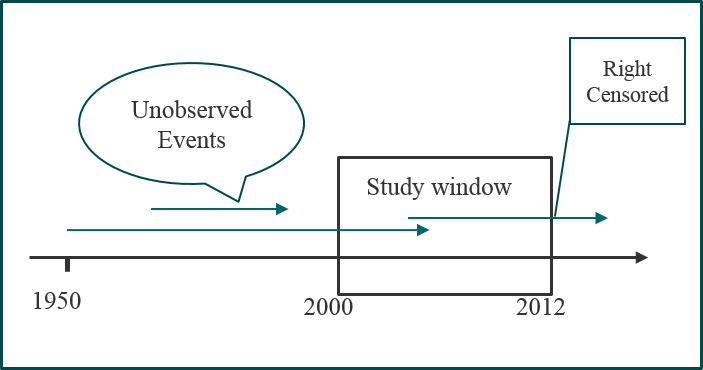
\includegraphics[width=3.5in]{fig1.png}
 	\caption{Right censor and left truncation}
 	\label{fig:1}
 \end{figure}
  Let $T$ denotes the time of main event of interest to occur and let $C$ denotes the end time of study. An observation is right censored when $T> C$, indicating the study do not have the failure time of the right censored observation. In this study, the study window is from November 2000 to December 2012 as shown in the figure \ref{fig:1}. Thus, the current active employees have unknown terminated date. They are treated as right censor. These right censored observations require special treatment in survival analysis: a censor indicator variable is created:
 \begin{align*}
 	\delta_i&=
 	\begin{cases}
 		1   &\text{if  }  t_i \leq c_i \text{ (uncensored),}\\
 		0   &\text{if  }  t_i > c_i \text{ (censored),}
 	\end{cases}
 \end{align*}
 where, $i$ denotes the ith observation, and the failure time of event for ith observation is minimum time between $t_i$ and $c_i$, i.e., $min(t_i, c_i)$, that is when $ c_i <t_i $, $c_i$ is taken as end time of the ith observation in order to do next  analysis.

 Left truncation is that the occurrence of an intermediate event prior to the event of interest appear in the sample dataset. Let $T$ denotes the time of event of interest to occur and let $X$ denotes the time an individual enters the study, that is time of truncation events occurs. Only the individuals with $T \geq X$ are observed in the study window. Left truncation in this study occurs due to no records for employees leaving the organization before November 2000 as unobserved events shown in the figure \ref{fig:1}. The left truncation leads to another bias. As shown in the figure \ref{fig:1}, the longest arrow represents a life span for an employee hired in 1950 and left in 2006. Those employees who remain in the study window increase the apparent lifetimes. The existence of truncation in the data must be taken into account in order to overcome this bias and to achieve accurate estimation of survival analysis \citep{carrion2010}. Let $t_{i0}$ denotes the start time of the ith observation, i.e., hired time or age at hired of ith employee, $x_{i}$ denotes the entry time of the ith observation, i.e., the start time of study (November 1st, 2000) or age at November 1st, 2000. The start time of the observation is maximum value between $t_{i0}$ and $x_i$, that is when $t_{i0} < x_i $, $x_i$ is taken as start time of the ith observation in order to eliminate the left truncation bias \citep{allison1995}. The number of failures in the $t_j$ is redefined for left truncation. When $x_i < t_j \le t_i$, the observation is in the risk set. When $t_{j} < x_i \le t_i$, the ith observation has not entered study yet at $t_j$ and it cannot be considered in the risk set. When $x_i \le t_i < t_j$, it indicates the ith observation whose failure time before $t_j$, and it cannot be considered in the risk set at time $t_j$ neither \citep{carrion2010}.

% simulation study.

\subsection{Cox PH regression model}
%   1. what is cox ph regression model.
Cox proportional hazards (PH) regression is a widely used method for estimating survival life events, introduced in a seminal paper by \citet{cox1972}. The Cox PH model is usually taken the form of hazard model formula as shown in the equation \ref{eq:cox}:
   \begin{equation}
   \label{eq:cox}
   h(t,x)=h_0(t)e^{(\sum_{i=1}^{k}\beta_ix_i)}
   \end{equation}

   where $x=(x_1, x_2, \ldots, x_k)$, $h_0(t)$ is the baseline hazard occurring when $x=0$, $\beta$ is the coefficients of $x$.
%    why not parametric. baseline cannot fit to any parametric model\\
%    2. cox regression without/ with time dependent variable\\
   The model provides a hazard expression at time t for an individual with a given specification of a set of explanatory variables denoted by the $x$. The Cox PH formula is the product of quantities at hazard time $t$: $h_0 (t)$ as the baseline hazard function and the exponential expression to the linear combination of $\beta_i x_i$, $x$ does not involve time $t$, so it is time-independent covariates. $x$ can also be time-dependent covariates, which named extended Cox PH regression as discussed in the section \ref{sec:coxt}. The key assumption for Cox PH regression model is proportion hazards. However, Cox regression can handle non proportional hazards using time-dependent covariate or stratification.
   The Cox PH regression is "robust" and popular, because the baseline hazard function $h_0 (t)$ is an unspecified function and its estimation can closely approximate correct parametric model \citep{kleinbaum1998}. Taking the logarithm of both sides of the equation, the Cox PH model is rewritten in the equation \ref{eq:coxlog}:
   \begin{equation}
   \label{eq:coxlog}
   \log{h(t,x)}=\alpha(t)+\sum_{i=1}^{k}\beta_ix_i
   \end{equation}
   where $\alpha(t)=\log{h_0(t)}$. If $\alpha(t)=\alpha$, the baseline is exponential distribution. In the Cox PH regression, $\alpha(t)$ do not limited on specific parametric distributions and it can take any form. The partial likelihood method is used to estimated $\beta$ coefficients of the Cox model without having to specify the baseline \citep{allison1995}. The Cox PH model is performed by SAS.


\subsection{Time dependent covariate and counting process}
\label{sec:coxt}
A time dependent covariate is that a covariate is not constant through the whole study and its value changes over the course of the study. The extended Cox PH regression model incorporates both time-independent and time-dependent covariates as shown in the equation \ref{eq:timecovar}:
\begin{equation}
\label{eq:timecovar}
h(t,x)=h_0(t)e^{(\sum_{i=1}^{k_1}\beta_ix_i+\sum_{j=1}^{k_2}\gamma_jx_j(t))}
\end{equation}
where $x=(x_1, x_2, \ldots, x_{k_1}, x_1(t), x_2(t), \ldots, x_{k_2}(t))$, $h_0(t)$ is the baseline hazard occurring when $x=0$, $\beta$ and $\gamma$ are the coefficients of $x$.
There are two time dependent covariates in this study: policy and economic indicators. Policy is to handle the downsizing policy issued in January 2008 with three months response time window to accommodate a voluntary reduction in force from the organization. Policy is a dummy variable across years:
\begin{align*}
Policy&=
\begin{cases}
1   &\text{if employee works in year 2008,}\\
0   &\text{if  employee does not work in year 2008.}
\end{cases}
\end{align*}

%What is counting process.   \\
Counting process method in SAS programming statements is used to handle time dependent covariates, which is each employee have multiple records. Each record is related to a time interval and the covariates in this record remain constant.
Therefore, Each employee has up to 3 records: before 2008, in-between 2008, and after 2008. Two variables, age, year of service, are used for repenting two time terminals of each interval or record. For age, one time point is age at beginning of the certain period, named "age at start"; and the other one is age at end of the curtain period, named "age at end".
    Two year of services points are also generated for each record: one is year of service at the beginning of the period, named "YCS at start"; the other one is the year of service at the end of the period, named "YCS at end".\\

Economic indicators is another time dependent covariates. Because economic indicators are fluctuated across the year, all the employees have up to 12 years records based on the calender year, which interval starts from hired date or January 1, and ends at terminated date or December 31 of certain year during the study window as shown in equation . The economic indicators are taken the average value for each year into the optimal model identified from the internal covariates to examine their impacts on turnover.
\begin{equation}
\label{eq:interval}
\begin{split}
(\text{start point}, \text{end point})= (max(\text{hired date}, \text{January 1 of a certain year}),\\
                                        min(\text{terminated date}, \text{December 31 of a certain year}))
\end{split}
\end{equation}

\subsection{Stratification model}
%I. what is stratification model;\\
An alternative for handling nonproportional hazards is stratification.  A stratified model allows each subgroup of data as defined by a grouping variable to have its own baseline hazard while sharing parameters for other covariates across. If the proportional hazards assumption holds within these subgroups then this model allows us to get valid common estimates of covariate effects using all of the observations. Equation \ref{eq:strata} below represents the hazard function for strata {\it z}; 
\begin{equation}
	\label{eq:strata}
	h(t,x,z)=h^z_0(t)e^{(\sum_{i=1}^{k}\beta_ix_i)}
\end{equation}
where $z$ represents the grouping variable, and $h^z\sigma_0(t)$ is a baseline hazard based for stratam z and $\beta_i$ are common effects of covariates ac. Note that the strata covariates cannot be the covariates in the Cox PH model.

%II. how to select a stratify variable\\
The proportional hazard assumption can be tested using Schoenfeld residuals which works even if the model includes time-dependent covariates; see \citet{allison2010,collett1994}. An alternative is to test the interaction between time-dependent and time-independent covariates in the Cox PH model. The assumption is valid if the interaction is not statistically significant ($P>0.05$).  Including a stratified covariate, when appropriate, can improve the Cox model's performance.  The C-statistic is used to compare models with and without stratification with a higher C value indicating a better model \citep{lemke2012}.

\subsection{Competing risks}
%  what is competing risks. competing ricks can help forecasting employee retirement and voluntary quit. \\
%  why select these two reasons to model.\\
  A competing risk is an event whose occurrence either precludes the occurrence of the event of interest or fundamentally alters the probability of occurrence of this event of interest \citep{tableman2003}. For example, turnover causes of an employee are exclusive and independent, i.e. an employee can experience only one event such as voluntary quit rather than retirement. This alters the probability of experiencing the event of interest, like retirement. Such events are known as competing risks events where one event of several different types of possible events can occur and hence the survival analysis for each event is calculated separately with the other events set as censored. Two mutually exclusive causes: retirement and voluntary quit are considered as the event of interests for each employees in this study, and the other events are treat as censored.

  There are several reasons for selecting these two causes. One main reasean is because the organization are interested in forecasting the turnover of retirement and voluntary quit. There are $1/3$  employees in that organization are over 50 years old who are eligible for retirement. The employee who voluntary quit usually is the one organization would like to keep \citep{allen2010}. And also voluntary quit costs highly for the organizations and firms \citep{selden2000}. Finally, the other reasons of turnover, such as layoff, transfer, death, or disability are caused by the factors which occurrence are random and hard to predict. The Cox PH regression for competing risks as shown in equation \ref{eq:competing}:
  \begin{equation}
  \label{eq:competing}
  h_j(t,x)=h_{j0}(t)e^{(\sum_{i=1}^{k}\beta_{ij}x_i)}
  \end{equation}
  where, $x_{j}$ is the covariate for a specific type of turnover. Note that the coefficient $\beta$ is the effects of the covariates may be different from different turnover types. If $\beta_{ij}$  is the same for all j, the model simplified to Cox PH model as shown in equation \ref{eq:cox}.


\subsection{Variable selection}
All the covariates are putting into Cox PH regression model and selected by manually backwards selection method based on $P<0.05$.  The variable selection procedure is as follow: first, all the covariates are used to build the model. Second, remove the non-significant variable ($P>0.05$) with the largest P value, and rerun the model with the other variables. Then, repeat the second step until there is no significant variable remaining in the model.
\subsection{Model evaluation and comparison}
%\subsubsection{Measurements}
%AIC, BIC, MAPE, c statistic.\\

The Cox PH model is evaluated by four statistics criteria:  Akaike’s information (AIC), Schwartz’s Bayesian criterion (SBC), C-statistics, and mean absolute percentage value (MAPE). The optimal model should have low AIC, SBC, and MAPE value, and high C-statistics for both training and holdout dataset. In this study, the model performance on holdout dataset is considered more important than that on the training dataset.  AIC and SBC are both information criteria using likelihood value. Usually, the best model comes with lowest AIC or SBC values. AIC, SBC values are automatically generated by the models.

C-statistics or the area under the receiver operating characteristic (ROC) curve is to test whether the probability of predicting the outcome is better than chance. It ranges from 0.5 to 1.  Models are considered acceptable when the C-statistic is higher than 0.7 \citep{hosmer2013}. C-statistics are calculated by using the predicted failure probability compared with the actual outcomes by SAS proc logistic. The predicted failure (retirement or voluntary quit) probability is actually the conditional failure probability for an employee at time $t_j$, given that the employee is active at time $t_{j-1}$. It is calculated based on the baseline and coefficients from Cox PH models for both training and holdout dataset as shown in equation \ref{eq:prob}.
\begin{equation}
\label{eq:prob}
\begin{split}% to allgin the equation
P\{t_{j-1}<T<t_j\} &=1-P\{T>t_j|T \ge t_j\}\\
&=1-\frac{S_{t_j}}{S_{t_{j-1}}}   \\
&=1-\frac{{S_0(t_j)}^{(\sum_{i=1}^{k}\beta_ix_i)}}{   {S_0(t_{j-1})}^{(\sum_{i=1}^{k}\beta_ix_i)}}
\end{split}
\end{equation}
where, $T$ is survival time, $t_j$ is a specific value for $T$, $S_0(t)$ is the baseline function generated by Cox PH model, $x$ is the covariates, and $\beta$ is the coefficient.

MAPE is another measure for comparing the accuracy of the model fitting between different forecast models since it measures relative performance \citep{chu1998} as shown in the equation \ref{eq:mape}.
\begin{equation}
	\label{eq:mape}
	MAPE=\sum_{t=1}^{n}\left | \frac{y_t-\hat{y_t}}{y_t} \right |\frac{1}{n}\%
\end{equation}
MAPE is calculated by using the yearly actual and predicted retirement or voluntary quit number as $y_t$ and $\hat{y_t}$, respectively.
The predicted retirement or voluntary quit number is the expected retirement or voluntary number summarized by aggregating all the failure probabilities for the active employees in the risk set at $t_j$ as shown in \ref{eq:expturnover}.
\begin{equation}
\label{eq:expturnover}
E(\text{turnover number at } t_j)=\sum_{i=1}^k{P_i\{t_{j-1}<T<t_j\}}
\end{equation}
where, $i$ denotes the ith employee.
%%%%%%% need some explain for traing and holdout mape%%%%%%%%%%%
The logistic regression and time series moving average methods are also employed to compare with the  performance of Cox PH regression model by MAPE value.
%The evaluation step is to calculate the yearly predicted turnover number for training and holdout dataset, and then compared the predicted number with the actual number.


%add evaluation formula.

%\subsubsection{Model validation}
% 1. Forecast employee turnover   how to forecast and calculate employee turnover number\\
% 2. conditional probability (The prediction is conditional probability): given the employee is survival at last year, what is the probability they survival or quit for this year.\\
% 3. the total number of employee turnover is the aggregate all turnover probabilities of employees at each year\\
%
% 4. split data into two ways: both training and holdout, training to build the model and holdout is to validate the model, and compare the actual vs forecasting, calculated MAPE and C statistics. \\
%       WAY1: training (10 years)and holdout (2 years). forecasting the total number of employee leaving the organization, compared to the actual number to calculate MAPE and C statistics. compare to logistic regression and time series methods to shown survival is better.\\
%       WAY2: random split the data into training (2/3) and holdout (1/3), using c statistics to select one best survival model.
 \subsection{Simulation on right censor and left truncation}
 
 In order to understand the performance and efficiency of the Cox PH model in right censored and left truncated data we perform a simulation study.
 
 Generated $n = 4000$ observations  from a a Weibull regression model  with one covariate which we referred to as age.  
 
 Age is uniformly distributed from 22 to 70 years of age, which is chosen to mimic the actual distribution of workers ages in our sample.
 
 In the regresion model, the coefficients for $\beta_age = -.025$ (Why?) and the coefficient for $\beta_0 = 1.5$. 
 
 The survival times $T_i$ are randomly generated from a Weibull distribution with shape parameter $\alpha$ and scale parameter $\lambda$, where $\alpha=1.5$ and $\lambda=exp(-0.025age+\beta_0)^{\frac{1}{\alpha}}$.
 
 
 The simulation is used to examine Cox PH model predictive performance with right censor and left truncation. The simulated lifetime data is generated based on the Weibull distribution. %The hazarld function for Weibull regression model with shape parameter $\alpha$, scale parameter $\lambda$, and covariate $X$ is shown in equation \ref{eq:weibul}, given $h_0=\alpha(\lambda)^\alpha t^{\alpha-1}$:
 %\begin{equation} \label{eq:weibul}
 %\begin{split}% to allgin the equation
 %h(t|X) & =h_0(t)exp(\beta X) \\
 %         &=\alpha (\lambda (exp(\beta X)^{\frac{1}{\alpha}})^\alpha t^{\alpha-1} \\
 %         &=\alpha(\tilde{\lambda} )^\alpha t^{\alpha-1}
 %\end{split}
 %\end{equation}
 %where, $\tilde{\lambda}=\lambda (exp(\beta X)^{\frac{1}{\alpha}}$.
 The simulation can be described as follows. The sample size was n=4000, with one variable $X$, named Age, which follows uniform distribution with parameter $a$ $(a=22)$ and $b$ $(b=70)$. Only one variable age is used in simulation process to make the estimation procedure simple and close to real world. The coefficient $\beta_{age}$ is taken $-0.025$ and $\beta_0=1.5$.
 Then, the survival time $T$ is random generated for each observation based on Weibull distribution with shape parameter $\alpha$ and scale parameter $\lambda$, where $\alpha=1.5$ and $\lambda=exp(-0.025age+\beta_0)^{\frac{1}{\alpha}}$.

 The simulation is performed on right censoring and left truncation separately, in order to observe the effects for different bias.
 For right censor simulation, the start point for all the observations are set as 0, and stop point is equal to the survival time $t_i$ for ith observation where $T=(t_1, t_2, \ldots, t_n)$. After that, a survival time histogram is generated. The censor time $C$ is set as first quarter, median, third quarter, and maximum of the survival time, respectively, to get 75\%, 50\%, 25\% and 0\% censoring proportions. When the survival time $t_i$ for ith observation is not greater than the censor time ($c_i$), the stop point is survival time and censor variable $\delta_i$ is 1. When survival time $t_i$ for ith observation is greater than censor time ($c_i$), the stop point is change to censor time ($c_i$) and censor variable $\delta_i$ is  0. The start point and the stop point are dependent variable in the cox regression model. $\delta$ is censor variable. And age is predictor or covariate. All these variables are applied to cox model using R EHA package.

 For left truncation simulation, the start point $U$ is generated as uniform distribution with $a=0$ and $b=max(T)$ which indicates an observation start randomly from time 0 to time $max(T)$. The stop point $S$ is $U+T$. The histogram is generated for $S$. The truncation time $L$ is set as 0, first quarter, median, and third quarter of $S$, respectively, to get 0\%, 25\%, 50\%, and 75\% truncation proportions. When start point $u_i$ for ith observation is less than truncation time $l_i$, the start point is reset as truncation time $l_i$. When start point $u_i$ for ith observation is not less than truncation time $l_i$, the start point does not change ($u_i$). In left truncation, the censor variable $\delta$ for all the observations are equal 1. All these variables are also used to build Cox PH model in R EHA package. The Cox PH model is conducted using "phreg" function in eha package and using weibull distribution to estimate the baseline for both right censoring and left truncation simulation. The "phreg" function performs Cox PH model and also provides a parametric baseline hazards estimation \citep{brostrom2012}. Total predicted failure number is calculated as shown in equation \ref{eq:prob} and \ref {eq:expturnover}. The actual and forecast failure number are plotted to compare the effects on different levels of bias.

 %accelarate model%
\section{Results}
\subsection{Right censor and left truncation simulation results}
\subsubsection{Right censoring simulation result}
The right censoring simulation result shows the average values of Cox PH model coefficient estimate and baseline parameter estimates for Weibull distribution based on 100 replication with the no censoring, 25\%, 50\%, and 75\% censoring proportion models as shown in Table \ref{table:rightcensor}. The events in the second column of the table indicate total failure events in the dataset without including censoring, which is $events=\sum_{i=0}^{4000}{\delta_i}$ where $\delta$ is censor variable. The coefficients of age for all four models are all close to 0.025, but it is over estimates (0.026) when high proportion of censoring (75\%) in the dataset. The overestimation is also shown by the estimates of shape parameter: the estimated value (1.539) for model with 75\% censoring is greater than $\alpha=1.5$. It underestimates the shape parameters when the censoring proportion is 25\% and 50\%, respectively. The most close estimation of shape is when there is no censoring in the data. The $-$log likelihood values decrease from low percentage censoring to high percentage censoring. Because the scale parameter is generated by the formula, there is no actual value of scale parameter to compare. However, compared to the estimated value from no censoring (2.668), the model overestimates with 25\% censoring (2.779), get close with 50\% censoring (2.675) and underestimates with 75\% censoring (1.539). The estimates decrease when the percentage of censoring increases. Overall, the estimates are close to actual simulated value when the censoring proportion is close to 50\%. However, it over- or under-estimates the coefficients when the censoring proportion is 75\%. The phenomenon is also verified by plotting the actual and predicted failure number in the figure \ref{fig:7}.  The red line is the actual failure number simulated by Weibull distribution. The dark blue line is the predicted failure number for the model with 75\% censoring which is higher than all the other three lines for predicted failure number before time 3.75 and overlaid with the other three lines after 3.75. The gap between this line and the others three lines reaches the largest value around time 1. The other three lines represent the predicted failure number from the model with no censor, 25\% censoring, and 50\% censoring, respectively. They are too close to be distinguished in the figure. Therefore, the right censoring simulation shows that the Cox PH model performs well and the estimates are close to the actual values when the censoring proportion is close to 50\%, and it deteriorates when the censoring proportion is 75\%, causing the overestimation of the total failure number.
% Table generated by Excel2LaTeX from sheet 'Sheet2'
% Table generated by Excel2LaTeX from sheet 'Sheet1'
\begin{table}[htbp]
	\renewcommand{\arraystretch}{1.5}
	\small
	\centering
	\caption{Right censoring simulation statistics}
	\begin{tabular}{ccrrrc}
		\hline
		\multirow{2}[2]{*}{Models} & \multirow{2}[2]{*}{Events} & \multicolumn{3}{c}{Variable estimate}  \\ \cline{3-5}
		
		&       & Age   & Scale & Shape &  \\\hline
		No Censor & 4000  & \multicolumn{1}{c}{0.0249} & \multicolumn{1}{c}{2.713} & \multicolumn{1}{c}{1.501}  \\
		25\% Censored & 3000  & \multicolumn{1}{c}{0.0248} & \multicolumn{1}{c}{2.709} & \multicolumn{1}{c}{1.500} \\
		50\% Censored & 2000  & \multicolumn{1}{c}{0.0246} & \multicolumn{1}{c}{2.673} & \multicolumn{1}{c}{1.506}  \\
		75\% Censored & 1000  & \multicolumn{1}{c}{0.0247} & \multicolumn{1}{c}{2.706} & \multicolumn{1}{c}{1.502}  \\
		\hline
	\end{tabular}%
	\label{table:rightcensor}%
\end{table}%
\begin{landscape}
	\begin{figure}[htbp]
		\centering
		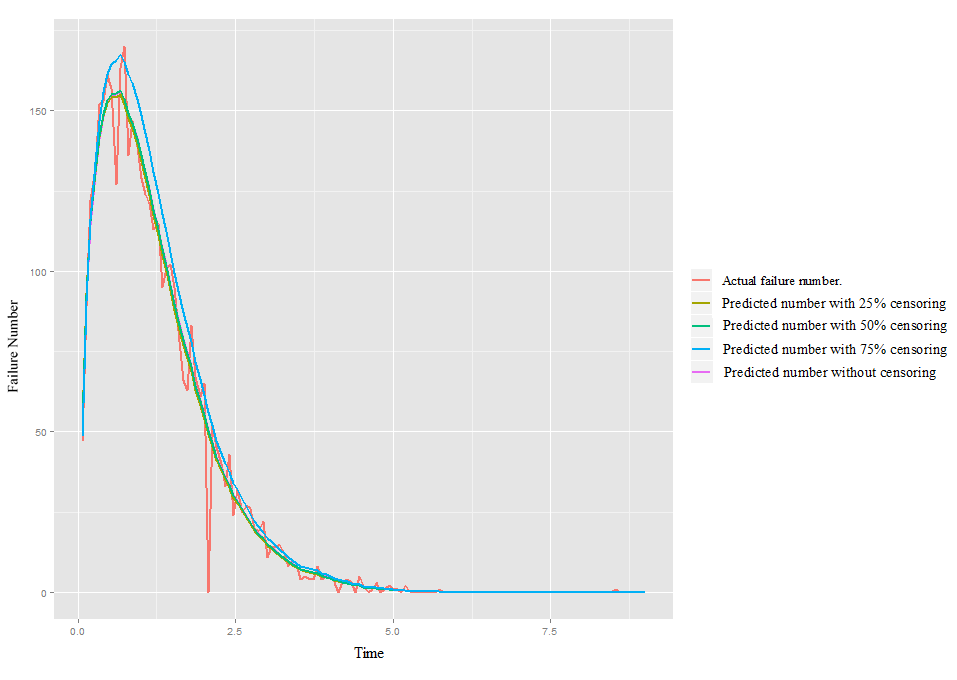
\includegraphics[width=9in]{Fig7}
		\caption{Actual vs. predicted failure number with various censoring}
		\label{fig:7}
	\end{figure}
\end{landscape}
% % % % % % % % % % % % % % % % % % % % % % % % %
% % % %Left truncation result % % % % % % % % % %
% % % % % % % % % % % % % % % % % % % % % % % % %
\subsubsection{Left truncation simulation results}
The left truncation bias simulation statistics for testing Cox PH model function shows the average values of coefficient estimate for age, baseline parameter estimates for scale and shape by Weibull distribution, and total predicted failure number based on 100 replications as shown in Table \ref{tab:lefttruncation}. The coefficients of age for all four models are all close to 0.025, even when high proportion of left truncation (75\%) in the dataset. The scale and shape parameter are also close for different portion of left truncation: the estimated values for scale are close to 2.7, and the estimated values for shape are close to 1.5, which are close to the true simulation value. However, The model overestimates the total failure number when left truncation proportion increasing. The last column is the summation of predicted failure number at a left truncation proportion. They are close to actual failure number (3993) when left truncation proportion is 0\%, which is 7 different. When left truncation reaches to 25\%, 50\%, and 75\%, the difference between the actual and predicted events increases from 16 to 34. 

However, the predicted failure number is smoothed and close to the actual one as shown in the figure \ref{fig:lefttruncation}. It is overestimates at the beginning of the time line when left truncation proportion is 50\% and 75\% as shown in figure \ref{fig:left50} and \ref{fig:left75}, where the dash lines are both higher than the solid lines at the beginning.
Therefore, the left truncation simulation test shows that the Cox PH model performs well when the censoring proportion is less than 50\%, and it deteriorates when the truncation proportion goes high causing the overestimation of the total failure number.
\begin{table}[h!]
	\renewcommand{\arraystretch}{1.5}
	\small
	\centering
	\caption{Left truncation simulation statistics}
	\begin{tabular}{ccccccc}
		\hline
		\multirow{2}[4]{*}{Model} & \multirow{2}[4]{*}{Events} & \multicolumn{3}{c}{Variable Estimates} & \multirow{2}{3cm}{Predicted Total Failure No.}  \\
		\cline{3-5} % \cline{i-j} partial horizontal line beginning in column i and ending in column j		
		&       & Age   & Scale & Shape &  &\\				
		\hline
		No left Truncation & 3999.5  & 0.0250 & 2.721 & 1.500  & 3993.38 \\
		25\%  left Truncation & 2999.8  & 0.0250 & 2.724  & 1.500  & 3016.20 \\
		50\%  left Truncation & 2000.1  & 0.0251 & 2.727 & 1.504  & 2033.10 \\
		75\%  left Truncation & 1000.1  & 0.0254 & 2.747 & 1.500  & 1034.45 \\
		\hline
	\end{tabular}%
	\label{tab:lefttruncation}%
\end{table}%
%negative loglikelihood value can be dropped. does not make sense.

\begin{figure}[h!]
	\centering
	\subfloat[No left truncation]{\label{fig:leftno}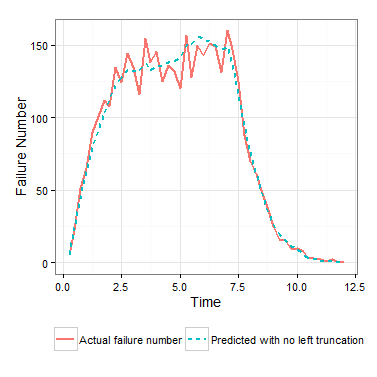
\includegraphics[width=2.75in]{notruncation.png}}
	\quad
	\subfloat[25\% left truncation]{\label{fig:left25}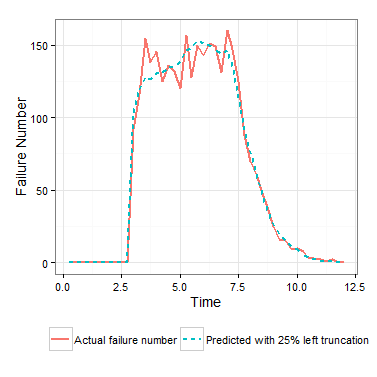
\includegraphics[width=2.75in]{25color.png}}
	\quad
	\subfloat[50\% left truncation]{\label{fig:left50}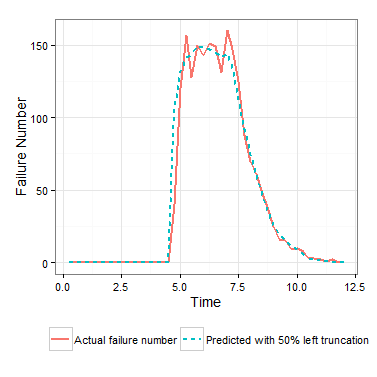
\includegraphics[width=2.75in]{50color.png}}
	\quad
	\subfloat[75\% left truncation]{\label{fig:left75}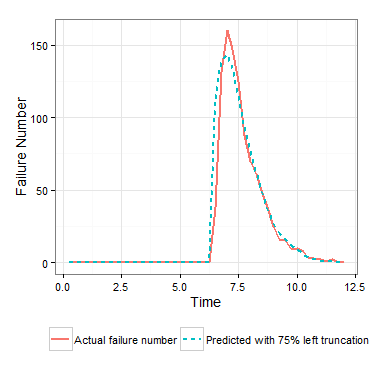
\includegraphics[width=2.75in]{75color.png}}
	\caption{Left truncation simulation results: actual vs. predicted failure number}
	\label{fig:lefttruncation}
\end{figure}

% 1- include the name of the package in the Results sections.  
% 2 - redo with results averaged over 100 data sets.
% 3 - explain concerns about censoring in our data.  About 50 % censored.  Large amount of truncation.
% 4) - Baseline can be highly variable in the extremes leading to poor 
% 5) Figures and discussion of coefficients and baseline estimates and impact on predictions.
% 6) Problems with PH in predictive modelling.  Truncation needs PH (is there another method)
%

\subsection{Retirement model without external variables}
   1. four survival model have been generated for comparison.
   2. significant variables.
   3. stratfication variable deterimation.
   4. model comparison based on validation way 1 and way2 (one table show all the models)
\subsection{Retirement model with external variables}
     best model and tested which variable does significantly impact on retirement.
\subsection{Voluntary quit model without external variables}
     I. dependent variable are YCSH, because age is not able to predict well.
     II. shorten the length of risk set.
     iii. model comparison. (survival model, time seris model, and logsitic regression model)
\subsection{Voluntary quit model with external variables}
    i. tested which variable does significantly impact on employee voluntary quit.


\section{Conclusions and Managerial Implications} 


	\bibliographystyle{abbrvnat}%Choose a bibliograhpic style%
	\bibliography{Bib}
\end{document}
